\documentclass{article}
\usepackage[utf8]{inputenc}
\usepackage{hyperref}
\urlstyle{same}
\usepackage{microtype}
\usepackage{graphicx}
\usepackage{graphicx}
\usepackage{tikz}
\usetikzlibrary{positioning}

\usepackage{color}

\definecolor{dkgreen}{rgb}{0,0.6,0}
\definecolor{gray}{rgb}{0.5,0.5,0.5}
\definecolor{mauve}{rgb}{0.58,0,0.82}
\definecolor{darkblue}{rgb}{0.0,0.0,0.6}
\definecolor{cyan}{rgb}{0.0,0.6,0.6}

\usepackage{listings,relsize}
\lstloadlanguages{R}
\lstset{ %
  language=R,                     % the language of the code
  basicstyle=\footnotesize,       % the size of the fonts that are used for the code
  numbers=left,                   % where to put the line-numbers
  numberstyle=\tiny\color{gray},  % the style that is used for the line-numbers
  stepnumber=1,                   % the step between two line-numbers. If it's 1, each line
                                  % will be numbered
  numbersep=5pt,                  % how far the line-numbers are from the code
  backgroundcolor=\color{white},  % choose the background color. You must add \usepackage{color}
  showspaces=false,               % show spaces adding particular underscores
  showstringspaces=false,         % underline spaces within strings
  showtabs=false,                 % show tabs within strings adding particular underscores
  frame=single,                   % adds a frame around the code
  rulecolor=\color{black},        % if not set, the frame-color may be changed on line-breaks within not-black text (e.g. comments (green here))
  tabsize=2,                      % sets default tabsize to 2 spaces
  captionpos=b,                   % sets the caption-position to bottom
  breaklines=true,                % sets automatic line breaking
  breakatwhitespace=false,        % sets if automatic breaks should only happen at whitespace
  title=\lstname,                 % show the filename of files included with \lstinputlisting;
                                  % also try caption instead of title
  keywordstyle=\color{blue},      % keyword style
  commentstyle=\color{dkgreen},   % comment style
  stringstyle=\color{mauve},      % string literal style
  escapeinside={\%*}{*)},         % if you want to add a comment within your code
  morekeywords={*,...}            % if you want to add more keywords to the set
} 

\setlength{\parskip}{5pt}
\begin{document}

\begin{titlepage}
    \begin{center}
    \line(1,0){300} \\
    [0.2in]
    \begin{flushleft}
    \huge{\bfseries{
Collective Bargaining 2.0}}\\ \Large{\textit{Streamlining the Negotiation Process through Natural Language Processing \& Machine Learning}}\\
    \end{flushleft}
    \line(1,0){200} \\
    [3.5cm]
    \end{center}
    \begin{flushleft}
    
    \textsc{\Large Ryan H. Gomez}\\
    [.5cm]
    
    \textsc{\large Michigan State University College of Law \\
    \normalsize Legal Analytics\\
    Spring 2015}\\
    [2cm]
    \textsc{\large Abstract}\\
    [.25cm]
    Contract clause identification promises to vastly reduce attorneys’ fees by decreasing the amount of review time. School district collective bargaining agreements are prime targets for clause identification since the contracts tend to be extremely long, renegotiated every few years, and clauses tend to be grandfathered in despite circumstances that make the clause no longer applicable. This study ultimately finds that collective bargaining agreements, as they are currently formatted, are not amenable to machine learning, and that more data cleaning is needed.\\
    [3.25cm]
    \small{$^\dagger$ \textit{A special thanks to all the California superintendents that responded to my (surely bothersome) mass email request.}} 
    \end{flushleft}
\end{titlepage}

\newpage
\section{Introduction}
\subsection{The Data}

The relevant population for this project consists of all school districts in California that have collective bargaining agreements (“CBA”) with the teacher’s union of that school district. Not every school district in California has an associated teacher’s union and CBA; however, most do. The CBAs are public documents, but schools are not required to report the contracts to any private or government entity. This presents unique challenges in gathering the CBAs from each school district that has one. 
	
In order to overcome the challenges associated with collecting each district’s CBA, I elected to use data available through California’s Department of Education in order to obtain an email list of each superintendent in California. This list includes every school in California, both active and closed, as well as schools without websites or contact information, which might indicate that it is either an incredibly small district or other issues. Using the dplyr package,\footnote{\hspace{2ex}Appendix 1.} I first selected variables that might be relevant to my search for school district contacts. I then further refined the data to only include unique school districts, since the district as a whole, rather than individual schools, contract with the associated teacher’s union. I then filtered that data by active school districts, districts that have websites, and districts that have email contact information for the superintendent. 
	
I was left with 988 school districts with superintendent email contacts, out of the 1,028 school districts in California.\footnote{\hspace{2ex}\textsc{California Dept. of Education,} \url{http://www.cde.ca.gov/ds/sd/cb/ceffingertipfacts.asp}, (last visited May 6, 2015).}  I then emailed all 988 superintendents requesting the CBA between the district and its teachers, and received 281 CBAs in response (28.4\% response rate). The CBAs came in a variety of file formats, some of which were scanned PDFs. In order to use the CBAs, I had to run OCR over them with Abbyy FineReader in order to get the each CBA into a machine-readable, plain HTML format that could be processed using the R program.\footnote{\hspace{2ex}For information on optical character recognition, \textit{see} \url{http://en.wikipedia.org/wiki/Optical_character_recognition}.}  Abbyy could not process several CBAs as they were password protected, and I ended up with 270 CBAs in total, or 26.2\% of all school districts in California.
	
In order to further process and clean the data, I placed the CBAs into a text corpus,\footnote{\hspace{2ex}For more information on text corpus, \textit{see} \url{http://en.wikipedia.org/wiki/Text_corpus}.}  transformed the contents to lowercase, removed numbers, punctuation and whitespace, and further removed stop words\footnote{\hspace{2ex}For information on stop words, \textit{see} \url{http://en.wikipedia.org/wiki/Stop_words}.} that appear within the tm package as well as stop words associated with HTML.\footnote{\hspace{2ex}\textit{See}, Figure 1 for a word cloud from all 270 CBAs.}  After cleaning preparing the corpus, I placed it into a document-term matrix.\footnote{\hspace{2ex}For more information on document-term matrices, \textit{see} \url{http://en.wikipedia.org/wiki/Document-term_matrix}.}

\subsection{Research Problem}

For this project, I wanted to explore the possibility of identifying clauses contained within a CBA that might indicate a unique attribute of the school district. For instance, certain school districts have “participative decision making” clauses that give teachers a voice in the development and improvement of instructional programs. School districts that have this clause in the CBA likely give more classroom autonomy to teachers, which might have discernible effects on each the school’s Academic Performance Index (“API”) scores.\footnote{\hspace{2ex}\textsc{California Dept. of Education}, \url{http://www.cde.ca.gov/Ta/ac/ap/} (last visited May 6, 2015).}

Being able to locate clauses that indicate unique attributes of a school district has both practical and academic implications. Academically, a school can be profiled based on certain clauses, and further research could be conducted to determine correlations with API scores, teacher autonomy, workplace satisfaction, or other important measures of school success. Practically, certain clauses might suggest an attribute of the school district that is no longer true, which in turn might suggest that the clause is superfluous. This could cut down attorney time by automatically identifying superfluous clauses, or by reducing negotiating time as the parties can focus on clauses that are actually applicable. 

In order to explore this idea, I used decision trees\footnote{\hspace{2ex}For information on how decision trees can be used for machine learning, \textit{see} \url{http://en.wikipedia.org/wiki/Decision_tree_learning}.} through the package \texttt{rpart} in order to predict whether a CBA contained a certain clause or not. The three clauses that I sought to predict were: presence or absence of a side letter agreement, presence or absence of a professional workday, and presence or absence of a defined workday. 

\section{Results \& Methods}
\subsection{Side Letter Agreements}
Side letter agreements are clauses that are not part of the primary CBA, but are nonetheless important to the parties. For example, Evergreen Elementary School District in San Jose, CA includes a side letter agreement concerning participative decision-making. The presence or absence of a side letter agreement can reflect difficulty in the bargaining process, or may reflect policies that are important to the parties, but are not traditionally within the scope of a CBA. Side letters  likely reflect pain points within a district, and might suggest areas that either side may press to gain a strategic advantage during the negotiation process. 

In order to detect side letter agreements, I first tokenized\footnote{\hspace{2ex}For more information on tokenization, \texit{see} \url{http://en.wikipedia.org/wiki/Tokenization_(lexical_analysis)}.} the text corpus and removed 99\% of the sparse terms. Since decision trees are a supervised learning method,\footnote{\hspace{2ex}For information concerning supervised learning methods in machine learning, \textit{see} \url{http://en.wikipedia.org/wiki/Supervised_learning}.} I then identified, via keyword search for “sideletter” and “side letter,” CBAs that contained a side letter agreement. The CBAs that contained a side letter clause were put into a vector named \texttt{sideletter} in order to label data that contained the clause I was looking for. The vector was then added to the data frame containing the tokenized corpus as \texttt{sideletterpresence}. The data frame was then split into training (70\% of the documents) and test sets (30\% of the documents).

A recursive partitioning function,\footnote{\hspace{2ex}For information on recursive partitioning, \textit{see} \url{http://en.wikipedia.org/wiki/Recursive_partitioning}.} \texttt{rpart}, was then used to predict the dependent variable, \texttt{sideletterpresence}, while using the remaining non-sparse terms as independent variables. My initial results used 10 documents to train the classifier and were output to a confusion matrix; the model has an accuracy rate of 93.8\%:

\begin{center}
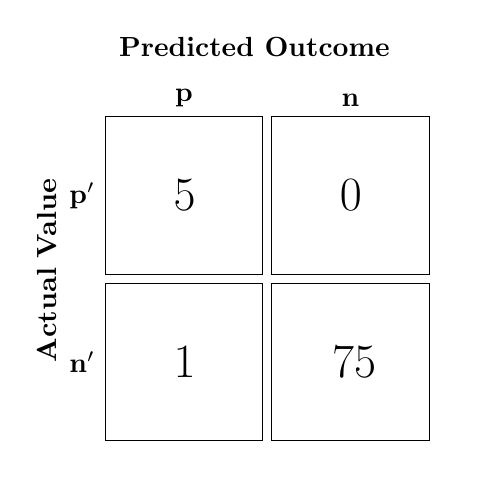
\begin{tikzpicture}[
box/.style={draw,rectangle,minimum size=2cm,text width=1.5cm,align=left}]
\matrix (conmat) [row sep=.1cm,column sep=.1cm] {
\node (tpos) [box,
    label=left:\( \mathbf{p'} \),
    label=above:\( \mathbf{p} \),
    ] {\hspace{5mm} \LARGE 5};
&
\node (fneg) [box,
    label=above:\textbf{n},
    label=right:\( \mathrm{} \)] {\hspace{5mm} \LARGE 0};
\\
\node (fpos) [box,
    label=left:\( \mathbf{n'} \),
    label=below:] {\hspace{5mm} \LARGE 1};
&
\node (tneg) [box,
    label=right:\( \mathrm{} \),
    label=below:] {\hspace{4mm} \LARGE 75};
\\
};
\node [rotate=90,left=.05cm of conmat,anchor=center,text width=2.5cm,align=center] {\textbf{Actual Value}};
\node [above=.05cm of conmat] {\textbf{Predicted Outcome}};
\end{tikzpicture}
\end{center}
The results suggest that the model is over-fitting, as I know there are more documents that contain side letter agreements. I ran the model a second time using 60 documents to train the classifier; the model has 100\% accuracy:\footnote{\hspace{2ex}Appendix 2.}
\begin{center}
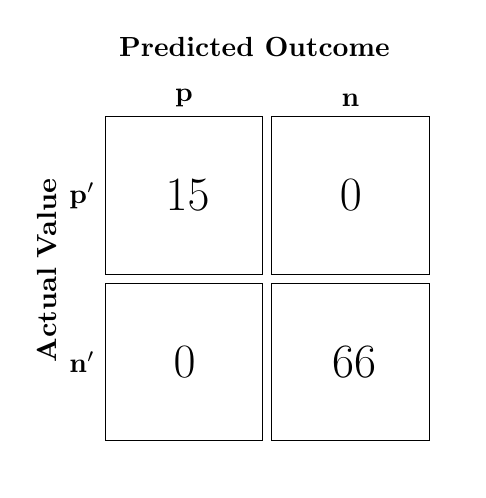
\begin{tikzpicture}[
box/.style={draw,rectangle,minimum size=2cm,text width=1.5cm,align=left}]
\matrix (conmat) [row sep=.1cm,column sep=.1cm] {
\node (tpos) [box,
    label=left:\( \mathbf{p'} \),
    label=above:\( \mathbf{p} \),
    ] {\hspace{4mm} \LARGE 15};
&
\node (fneg) [box,
    label=above:\textbf{n},
    label=right:\( \mathrm{} \)] {\hspace{5mm} \LARGE 0};
\\
\node (fpos) [box,
    label=left:\( \mathbf{n'} \),
    label=below:] {\hspace{5mm} \LARGE 0};
&
\node (tneg) [box,
    label=right:\( \mathrm{} \),
    label=below:] {\hspace{4mm} \LARGE 66};
\\
};
\node [rotate=90,left=.05cm of conmat,anchor=center,text width=2.5cm,align=center] {\textbf{Actual Value}};
\node [above=.05cm of conmat] {\textbf{Predicted Outcome}};
\end{tikzpicture}
\end{center}

Contrary to what 100\% accuracy suggests, the model is not performing as intended; it is likely over-fitting to random noise in the documents. I decided to try clauses pertaining to professional workdays or defined workdays. Since every CBA contains either a defined or professional workday, my thinking is that the model will have an easier time classifying the documents. 

\subsection{Professional Workday versus Defined Workday}

A professional workday is contrasted with a defined workday, and a CBA will dictate what sort of workday a district has. A professional workday gives teachers flexibility in when they report to and leave work, while a defined workday mandates the hours a teacher will work each day.  For example, one CBA mandates that the workday is “7:45 a.m. – 2:35 p.m.” The presence of a professional workday tends to reflect a district’s recognition of a teacher as a professional, and likely corresponds with greater teacher autonomy overall, while a defined workday likely reflects less teacher autonomy.

Since districts have either a professional workday or defined workday, I ran the classifier twice after tokenizing the corpus and removing 99\% of the sparse terms. The first run was aimed at identifying a professional workday as \texttt{1} and a defined workday as \texttt{0}, and the second run was aimed at identifying a defined workday as \texttt{1} and a professional workday as \texttt{0}.

In order to train the \texttt{rpart} classifier, I randomly selected individual CBAs and labeled the document according to the type of workday that was present. For professional workdays, I placed 14 CBAs into a vector called \texttt{profworkday}, and for defined workdays, I placed 16 CBA into a vector called \texttt{defworkday}. The vectors were then added to the data frame as \texttt{profworkdayclass} and \texttt{defworkdayclass}, and the classifiers were run separately. 

\pagebreak For \texttt{profworkdayclass}, the model was 100\% accurate:

\begin{center}
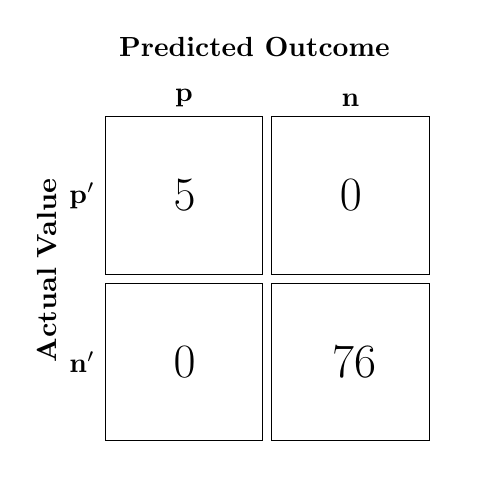
\begin{tikzpicture}[
box/.style={draw,rectangle,minimum size=2cm,text width=1.5cm,align=left}]
\matrix (conmat) [row sep=.1cm,column sep=.1cm] {
\node (tpos) [box,
    label=left:\( \mathbf{p'} \),
    label=above:\( \mathbf{p} \),
    ] {\hspace{5mm} \LARGE 5};
&
\node (fneg) [box,
    label=above:\textbf{n},
    label=right:\( \mathrm{} \)] {\hspace{5mm} \LARGE 0};
\\
\node (fpos) [box,
    label=left:\( \mathbf{n'} \),
    label=below:] {\hspace{5mm} \LARGE 0};
&
\node (tneg) [box,
    label=right:\( \mathrm{} \),
    label=below:] {\hspace{4mm} \LARGE 76};
\\
};
\node [rotate=90,left=.05cm of conmat,anchor=center,text width=2.5cm,align=center] {\textbf{Actual Value}};
\node [above=.05cm of conmat] {\textbf{Predicted Outcome}};
\end{tikzpicture}
\end{center}

For the \texttt{defworkdayclass}, the model was also 100\% accurate:

\begin{center}
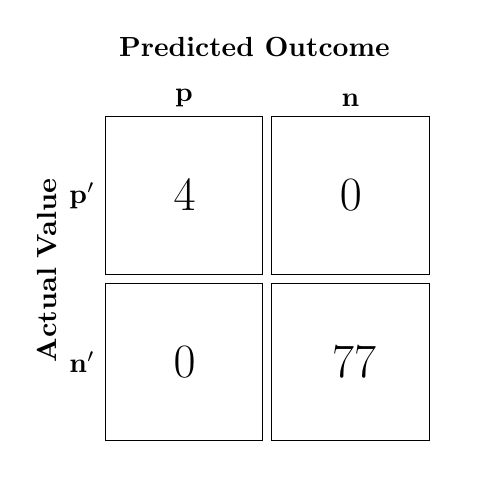
\begin{tikzpicture}[
box/.style={draw,rectangle,minimum size=2cm,text width=1.5cm,align=left}]
\matrix (conmat) [row sep=.1cm,column sep=.1cm] {
\node (tpos) [box,
    label=left:\( \mathbf{p'} \),
    label=above:\( \mathbf{p} \),
    ] {\hspace{5mm} \LARGE 4};
&
\node (fneg) [box,
    label=above:\textbf{n},
    label=right:\( \mathrm{} \)] {\hspace{5mm} \LARGE 0};
\\
\node (fpos) [box,
    label=left:\( \mathbf{n'} \),
    label=below:] {\hspace{5mm} \LARGE 0};
&
\node (tneg) [box,
    label=right:\( \mathrm{} \),
    label=below:] {\hspace{4mm} \LARGE 77};
\\
};
\node [rotate=90,left=.05cm of conmat,anchor=center,text width=2.5cm,align=center] {\textbf{Actual Value}};
\node [above=.05cm of conmat] {\textbf{Predicted Outcome}};
\end{tikzpicture}
\end{center}
Again, the model appears to be over-fitting to random noise. Contrary to my thinking that because each CBA has either a professional workday or defined workday the classifier will not pick up on as much noise,\footnote{\hspace{2ex}I ran the classifier a second time using more documents for \texttt{profworkday}, but ultimately saw no improvement. \textit{See}, Appendix 3.} it appears that I am still running into the same problems as with side letters. 
\section{Discussion}

All of the models suffer from severe over-fitting, and efforts to reduce over fitting ultimately had little effect. I attribute most of the over-fitting to the sheer amount of noise in the data. The CBAs were completely unstructured, with no obvious way to parse the text, as each district provides its own unique formatting for each document. On average, a CBA contains approximately 23,489.5 words,\footnote{\hspace{2ex}This was calculated via Terminal, after setting the working directory, with the command: \texttt{find . -type f -print0 | xargs -0 cat | wc -w}, which returned 6,342,165 words for 270 documents.} and the \textt{rpart} classifier is attempting to locate very specific clauses from each CBA. One would expect that the CBAs are, as a whole, very similar and address similar labor issues, despite also having unique clauses; a cursory look at random CBAs confirms that this is true. For this model, it means that the \texttt{rpart} algorithm is likely picking up on irrelevant variables, instead of the specific clause that I am looking for. 

This finding is largely confirmed by a proximity matrix that was created using the \texttt{bigrf} package.\footnote{\hspace{2ex}\textit{See} Figure 2 for proximity matrix.} This package uses random forests, or many decision trees as opposed to one, in order to classify the CBAs as having or not having a specified clause. A proximity matrix, which, broadly speaking, measures the similarity or dissimilarity between documents was then plotted. In the proximity matrix for \texttt{sideletterpresence}, we can visually see that the decision trees are finding irrelevant similarities and dissimilarities between documents that have side letter agreements and those that don’t. This is likely due to the large amount of noise in each document. 

Despite the problems with the data and model, my hypothesis---that by predicting which clauses a school district has in its CBA, we can characterize that school district---and the practical and academic implications that stem from that has been, at least partially, anecdotally, confirmed. Several superintendents that I spoke with during this study were able to confirm that they in fact have clauses in the district’s CBA that are not applicable to the district as it currently is. Moreover, superintendents also seem to agree that certain clauses, such as “participative decision making,” are essential for student success and workplace satisfaction, and further the government-backed, “teach to lead,” initiative.\footnote{\hspace{2ex}\textit{See} \textsc{U.S. Dept. of Education}, \textit{Teach to Lead: Advancing Teacher Leadership} (March 14, 2014), \url{https://www.ed.gov/news/speeches/teach-lead-advancing-teacher-leadership}.} 

Moving forward with this project will mostly involve formatting the CBAs in XML, which enables users to “tag” documents and then carry out tasks associated with those tags. Doing this should vastly reduce the amount of noise, since clauses could be specifically targeted, and similar clauses could then be identified and traced back to the document and district. Simply being able to target clauses, paragraphs, or even articles, would vastly improve this model’s performance.

\section{Conclusion}

Despite the severe limitations in this study, I believe this is a promising area for further research. Clause identification for contracts promises to greatly reduce attorney fees by decreasing the amount of time needed to manually review a 100+ page contract, and can allow the parties to quickly identify salient clauses. 

\newpage
\begin{center}
Figure 1\\
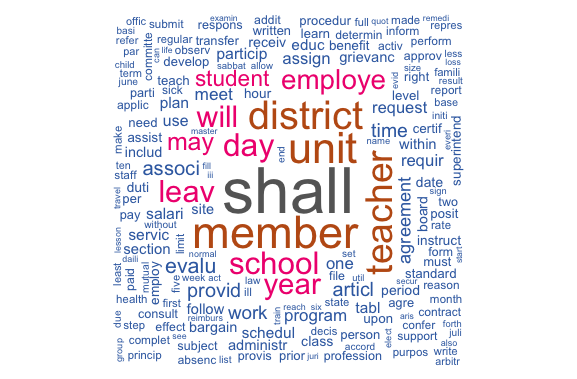
\includegraphics[width=\linewidth]{cloud.png}
\end{center}
\newpage
\begin{center}
Figure 2\\
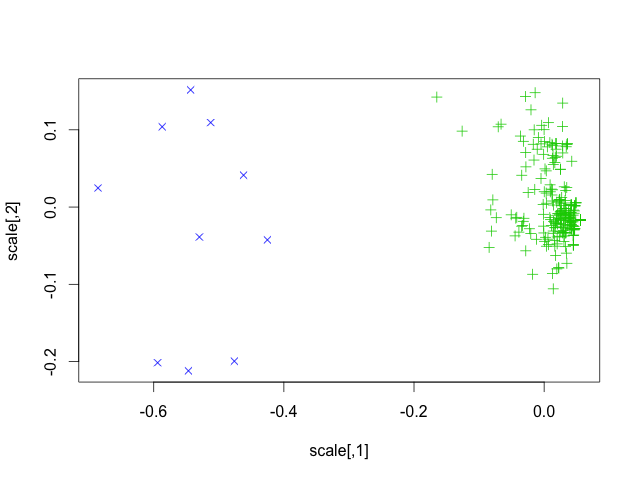
\includegraphics[width=\linewidth]{Rplot.png}
\end{center}

If the model were not picking up on the noise, we would expect to see some of the green + symbols closer to the blue x's. This is because at least some of the green +'s contain side letter agreements. 
\newpage
\begin{center}
Appendix 1
\end{center}

\begin{lstlisting}

library(dplyr)
# http://www.cde.ca.gov/ds/si/ds/pubschls.asp
ca_schools <- read.csv("Desktop/pubschls.csv")
ca_select <- select(ca_schools, StatusType, County, District, City, Phone, Website, AdmFName1, AdmLName1, AdmEmail1)
ca_unique_dist <- distinct(ca_select, District)
ca_subset <- filter(ca_unique_dist, StatusType == "Active")
ca_unique_dist <- ca_subset
ca_subset <- filter(ca_unique_dist, Website != "")
ca_unique_dist <- ca_subset
ca_adm_email <- filter(ca_subset, AdmEmail1 != "")

\end{lstlisting}
\newpage
\begin{center}
Appendix 2
\end{center}

\begin{lstlisting}
sideletter <- c("8-13-10_LAEA_combined.htm", "2011 11 28 .FCEAContract.htm", "2013-16 contract.htm", "2013-16_SEA_Agreement_ONLINE.htm", "2013-2016 DTA contract scanned and signed.htm", "2014 -15   edits  of BRSFA contract.htm", "2014-2016 Master Agreement.htm", "SVFT_Agreement_7-17-14.htm", "SEA-Teachers-Contract-2013-2016.htm", "EGEA_Contract_2013-2015.htm", "ATAcontract.htm", "EEEA Contract 2013-14, revised.htm", "2013-16_SEA_Agreement_ONLINE.htm", "5399260843028842110.htm", "4039315675021134549.htm", "SLTA Contract 2012-2015 Final.htm", "hr_cert_agreement.htm", "ata contract.htm", "Final 2014-2017 DTA CBA, based on 2011-13, Mar2015.htm", "CUTA_Agreement_2012-2013_through_2014-2015.htm", "BVTA Contract 2013-2016 (9-19-14).htm", "LSEA contract agreement 07-09.htm", "2013-16 contract.htm", "YCTA Contract.htm", "SDTA Agreement .htm", "PaloAlto.htm", "2011 11 28 .FCEAContract.htm", "PSEA CBA 2013-15 FINAL.1.htm", "BEA Contract 2012-2015 with Appendices.htm", "AeaContractUntil2012.htm", "8-13-10_LAEA_combined.htm", "4733679209303521488.htm", "MEA - Master Agreement 2014-2017.htm", "mhusd-mhft_contract_2012_-_2015_revised_july_1_2014_2.htm", "FMEA Contract 12-15 FINAL VERSION.htm", "RSD CTA 13-14 agreement.htm", "smcea-contract-2012-2015.htm", "GSCFT_2011_2014_Contract_revised_for_12_13_signature.htm", "HEA Contract 2013_2016_Appendices.htm", "Eureka 2014-15 Certificated Agreement (Contract) FINAL VERSION 9-12-14.htm", "3244577001150048049.htm", "4939176898569869228.htm", "272920477733032911.htm", "4899154045243849424.htm", "2013-2016 DTA contract scanned and signed.htm", "ACTA Contract July 1 2009 - June 30 2012 FINAL JUNE 2011.htm", "kceta_contract_7-1-14_to_6-30-17.htm", "LTA Collective Bargaining Agreement 2012-2015.htm", "https___doc-04-cc-apps-viewer.googleusercontent.htm", "MEA Agreement (2).htm", "CTA contract 7-1-13 o 6-30-14 rev.htm", "COMPLETE CBA RVTA 2013-16 changesthru6.30.15.htm", "UTA_CONTRACT_14-15.htm", "Evergreen.htm", "2014-2016 Master Agreement.htm", "SETA Agreement  FINAL 2013-16.htm", "Approved Opener Revisions 2012-2015 4-10-13.htm", "Certificated Contract 2013_2016_Board approved June 13_2013.htm", "J.C.T.A. contract 2010-2013.htm", "OUTA Contract 2011 to 2014.htm")
\end{lstlisting}
\newpage
\begin{center}
Appendix 3
\end{center}

\begin{lstlisting}
profworkday <- c("8-13-10_LAEA_combined.htm", "12-13 STEA Contract FINAL DRAFT  12-13-13.htm", "13-14 ACT Contract Final.htm", "13-14 Contract - With Settlement Agreement.htm", "14-15.CUEA.Contract.htm", "1408-agrmt-sbcta_12-15.htm", "2011 11 28 .FCEAContract.htm", "2011-2014 SWTA Contract.htm", "2012-13 MCTA Agreement PDF.htm", "2012-15_CEA_Contract.htm", "2013-16 contract.htm", "3244577001150048049.htm", "3350576201222205676.htm", "7543943393345802461.htm", "BEA Contract 2012-2015 with Appendices.htm", "BEA.htm", "contract 2014-2017.htm", "Evergreen.htm", "J.C.T.A. contract 2010-2013.htm", "MARFAC contract 2011-14 (FINAL) (1).htm", "scoeta_contract.htm", "SEA-Teachers-Contract-2013-2016.htm", "TAWC Contract - Master - 2011 - 2014.htm")
\end{lstlisting}
\newpage
\begin{center}
Appendix 4
\end{center}

\noindent All code may be found on GitHub at \url{https://github.com/ryangomez976/Legal_Analytics/tree/master/Final%20Project}.\\
[1mm]

\begin{lstlisting}

# Getting a TDM and predicting parties while retaining file names
library(XML)
library(SnowballC)
library(plyr)
library(class)
library(RCurl)
library(tm)
library(wordcloud)
library(RColorBrewer)
library(RWeka)
library(R.utils)
library(reshape2)
library(rpart)

# Creating and cleaning the corpus
corpus <- VCorpus(DirSource("~/Desktop/Legal_Analytics_Final/plain_html/"))
corpus <- tm_map(corpus, content_transformer(tolower))
corpus <- tm_map(corpus, removeNumbers)
myStopwords <- c(stopwords("english"), "p", "br", "td", "tr", "colspan", "d", "amp", "nbsp", "border", "<body>", "</body>", "<p>", "</p>")
corpus <- tm_map(corpus, removeWords, myStopwords)
corpus <- tm_map(corpus, stripWhitespace)
corpus <- tm_map(corpus, removePunctuation)
corpus_clean <- corpus

# Creating a word cloud for high-level overview of the corpus
corpus <- tm_map(corpus, stemDocument, language = "english")
tdm <- TermDocumentMatrix(corpus, control = list(wordLengths = c(3, 14)))
tdm_clean <- tdm
tdm <- removeSparseTerms(tdm, 0.50)
findFreqTerms(tdm, lowfreq = 1000)
matrix <- as.matrix(tdm)
wordFreq.sort <- sort(rowSums(matrix), decreasing=T)
pal <- brewer.pal(8,"Accent")
pal <- pal[-(1:4)]
word.cloud <- wordcloud(words = names(wordFreq.sort), freq = wordFreq.sort, min.freq = 1000, random.order = F, colors = pal)

# Finding "sideletter" clauses. A sideletter reflects terms that are important to the parties, but came to light outside of the normal bargaining process, or were important, but not important enough to include in the CBA.
options(mc.cores=1)
corpus <- corpus_clean
corpus <- tm_map(corpus, stemDocument, language = "english")

gram1Tokenizer <- function(x) {RWeka::NGramTokenizer(x, RWeka::Weka_control(min = 1, max = 1))}

tdm1 <- TermDocumentMatrix(corpus, control = list(tokenize=gram1Tokenizer, wordLengths = c(3, 14)))
tdm1 <- removeSparseTerms(tdm1, 0.99)

df <- as.data.frame(inspect(tdm1))
dft <- t(df)
dft <- data.frame(dft)
sideletter <- c("Evergreen.htm", "2013-16_SEA_Agreement_ONLINE.htm", "ACTA Contract July 1 2009 - June 30 2012 FINAL JUNE 2011.htm", "CUTA_Agreement_2012-2013_through_2014-2015.htm", "Eureka 2014-15 Certificated Agreement (Contract) FINAL VERSION 9-12-14.htm", "GSCFT_2011_2014_Contract_revised_for_12_13_signature.htm", "hr_cert_agreement.htm", "MEA - Master Agreement 2014-2017.htm", "SJTA COLLECTIVE BARGAINING CONTRACT_1416.htm", "SLTA Contract 2012-2015 Final.htm")
sideletterpresence <- c()
sideletterpresence <- c(sideletterpresence,(ifelse((rownames(dft) %in% sideletter), 1, 0)))
dft <- cbind(dft, sideletterpresence)
dft$class <- as.factor(dft$sideletterpresence)

set.seed(5983)
training <- sample(nrow(dft), ceiling(nrow(dft) * 0.7))
test <- (1:nrow(dft))[-training]
training <- dft[training,]
test <- dft[test,]

patree <- rpart(sideletterpresence ~ ., data=training, method = "class")
patree.predictions.eval <- predict(patree, test, type = "class")

confusionmatrix <- table(test$sideletterpresence, patree.predictions.eval)
confusionmatrix

tn <- confusionmatrix[1,1] #true negative
fp <- confusionmatrix[1,2] #false positive
fn <- confusionmatrix[2,1] #false negative
tp <- confusionmatrix[2,2] #true positive

accuracy.rate <- (tp + tn) / (tp + tn + fp + fn)
accuracy.rate

# Professional workday vs. defined workday. The presence of a professional workday clause likely indicates more autonomy for teachers, whereas a defined workday likely indicates less teacher autonomy. 
# 1 indicates a professional workday, 0 indicates a defined workday. This will be switched for another classification to observe any differences.
options(mc.cores=1)
corpus <- corpus_clean
corpus <- tm_map(corpus, stemDocument, language = "english")

gram1Tokenizer <- function(x) {RWeka::NGramTokenizer(x, RWeka::Weka_control(min = 1, max = 1))}

tdm1 <- TermDocumentMatrix(corpus, control = list(tokenize=gram1Tokenizer, wordLengths = c(3, 14)))
tdm1 <- removeSparseTerms(tdm1, 0.99)

df <- as.data.frame(inspect(tdm1))
dft <- t(df)
dft <- data.frame(dft)
profworkday <- c("2012-13 MCTA Agreement PDF.htm", "2013-16 contract.htm", "3244577001150048049.htm", "3350576201222205676.htm", "7543943393345802461.htm", "BEA Contract 2012-2015 with Appendices.htm", "BEA.htm", "contract 2014-2017.htm", "Evergreen.htm", "J.C.T.A. contract 2010-2013.htm", "MARFAC contract 2011-14 (FINAL) (1).htm", "scoeta_contract.htm", "SEA-Teachers-Contract-2013-2016.htm", "TAWC Contract - Master - 2011 - 2014.htm")

profworkdayclass <- c()
profworkdayclass <- c(profworkdayclass,(ifelse((rownames(dft) %in% profworkday), 1, 0)))
dft <- cbind(dft, profworkdayclass)
dft$class <- as.factor(dft$profworkdayclass)

set.seed(5983)
training <- sample(nrow(dft), ceiling(nrow(dft) * 0.7))
test <- (1:nrow(dft))[-training]
training <- dft[training,]
test <- dft[test,]

patree <- rpart(profworkdayclass ~ ., data=training, method = "class")
patree.predictions.eval <- predict(patree, test, type = "class")

confusionmatrix <- table(test$profworkdayclass, patree.predictions.eval)
confusionmatrix

tn <- confusionmatrix[1,1] #true negative
fp <- confusionmatrix[1,2] #false positive
fn <- confusionmatrix[2,1] #false negative
tp <- confusionmatrix[2,2] #true positive

accuracy.rate <- (tp + tn) / (tp + tn + fp + fn)
accuracy.rate

# 1 indicates a defined workday, 0 indicates a professional workday.
options(mc.cores=1)
corpus <- corpus_clean
corpus <- tm_map(corpus, stemDocument, language = "english")

gram1Tokenizer <- function(x) {RWeka::NGramTokenizer(x, RWeka::Weka_control(min = 1, max = 1))}

tdm1 <- TermDocumentMatrix(corpus, control = list(tokenize=gram1Tokenizer, wordLengths = c(3, 14)))
tdm1 <- removeSparseTerms(tdm1, 0.99)
df <- as.data.frame(inspect(tdm1))
dft <- t(df)
dft <- data.frame(dft)
defworkday <- c("4733679209303521488.htm", "5724342063445673460.htm", "7679200709597512380.htm", "APT-PUSD AGREEMENT 2014-2016-FINAL.htm", "cba020711.htm", "Certificated Contract 2013_2016_Board approved June 13_2013.htm", "FINAL_2015__2013-2016_Ratified_TTA_Contract.htm", "GSCFT_2011_2014_Contract_revised_for_12_13_signature.htm", "LSEA contract agreement 07-09.htm", "mhusd-mhft_contract_2012_-_2015_revised_july_1_2014_2.htm", "NTA-Contract-July-1-2014-June-20-2016-FINAL.htm", "PVTA Contract 2013-2016 FINAL.htm", "SDTA Collective Bargaining Agreement 2013-16.htm", "Tulare_CertificatedMasterContract20142017_020415.htm", "Woodville  teacher Contract  12-13.htm", "YCTA Contract.htm")

defworkdayclass <- c()
defworkdayclass <- c(defworkdayclass,(ifelse((rownames(dft) %in% defworkday), 1, 0)))
dft <- cbind(dft, defworkdayclass)
dft$class <- as.factor(dft$defworkdayclass)

set.seed(5983)
training <- sample(nrow(dft), ceiling(nrow(dft) * 0.7))
test <- (1:nrow(dft))[-training]
training <- dft[training,]
test <- dft[test,]

patree <- rpart(defworkdayclass ~ ., data=training, method = "class")
patree.predictions.eval <- predict(patree, test, type = "class")

confusionmatrix <- table(test$defworkdayclass, patree.predictions.eval)
confusionmatrix

tn <- confusionmatrix[1,1] #true negative
fp <- confusionmatrix[1,2] #false positive
fn <- confusionmatrix[2,1] #false negative
tp <- confusionmatrix[2,2] #true positive

accuracy.rate <- (tp + tn) / (tp + tn + fp + fn)
accuracy.rate

\end{lstlisting}

\end{document}
